\documentclass{chi2005}
\usepackage{times}
\usepackage{cite}
\usepackage[german]{babel}  % for a few German characters used in the text
\usepackage{hyperref}
\usepackage{color}
\usepackage{listings}
\usepackage{graphicx}
\lstset{ %
language=Ruby,                % choose the language of the code
basicstyle=\footnotesize,       % the size of the fonts that are used for the code
numbers=left,                   % where to put the line-numbers
numberstyle=\footnotesize,      % the size of the fonts that are used for the line-numbers
stepnumber=1,                   % the step between two line-numbers. If it is 1 each line will be numbered
numbersep=5pt,                  % how far the line-numbers are from the code
backgroundcolor=\color{white},  % choose the background color. You must add \usepackage{color}
showspaces=false,               % show spaces adding particular underscores
showstringspaces=false,         % underline spaces within strings
showtabs=false,                 % show tabs within strings adding particular underscores
frame=single,           % adds a frame around the code
tabsize=2,          % sets default tabsize to 2 spaces
captionpos=b,           % sets the caption-position to bottom
breaklines=true,        % sets automatic line breaking
breakatwhitespace=false,    % sets if automatic breaks should only happen at whitespace
}

\pagenumbering{arabic}  % Arabic page numbers

\title{Comparison of Algorithms for Searching Strings}
\numberofauthors{1}
\author{Adam Sinnett}

\clubpenalty=10000
\widowpenalty=10000
\tolerance=1000

\begin{document}
\maketitle

\abstract{In this paper we describe the class of algorithms used in string searching and compare the time and space complexity amongst several different algorithms. We begin with the naive brute force method, and then examine the improvements offered by Knuth-Morris-Pratt, Boyer-Moore and Rabin-Karp.}

\keywords{String Searching, Boyer-Moore,  Rabin-Karp, Knuth-Morris-Pratt}

\section{I. Introduction}

String searching is a problem that comes up often in the creation of computer programs. It has wide uses from text editors, to DNA matching and search engines. In this paper I will present four methods of accomplishing this task, and examine their complexity in both time and space for efficiency. I have implemented and tested these algorithms in the ruby programming language. Programs written in this language are easy to follow those who don't know the language, and it provides clear domain-specific languages(dsl) for testing and profiling the code. Specifically, testing was done with the rspec framework and profiling with the ruby-profile tool on the REE vm. Using this configuration for profiling allows one to disable garbage collection for the duration of the test, providing accurate measurement of time and space. All code and ancillary materials can be found at \url{http://github.com/quandrum/CS350-Project}

\section{II. Background Material}

String searching can be formalized as follows. Assume we have a text as an array T[1..n] of length n and a pattern as an array P[1..m] of length m $\le$ n. We can further assume the elements of these arrays are members of some finite alphabet $\Sigma$. We can then say P occurs with shift \emph{s}  in T if $0 \le s \le n - m$ and T[\emph{s+j}] = P[\emph{j}] for $1 \le j \le m$. If P occurs with shift \emph{s} in T, then \emph{s} is a valid shift. When attempting to match P to a section of T, we shall call that section of T the window. String searching is the problem of finding all valid shifts with which a given pattern \emph{P} occurs in a given text \emph{T}. For the purpose of this paper, we will only consider the problem of finding the first such valid shift. 

\subsection{a. Preprocessing}

Of the four strategies for string searching we will consider, three use some form of preprocessing the pattern. This will divide our algorithms into two steps, which we shall call preprocessing and matching. We will see by extracting information about the pattern before hand and using that knowledge in the matching stage, there can be significant increases in the time efficiency of our matches. However, these strategies also increase our space efficiency, and each implementation will have to consider this trade-off.

\section{III. Searching with Brute Force Strategy}

\subsection{a. Description}

The naive method of string search is quite obvious. We shall align our pattern \emph{P} with the first m characters and start matching the each character in \emph{T} and \emph{P} in order. If we find m matching pairs of characters, then we have found a valid shift. If we find a mismatching pair, we shift the start of our matching one character to the right and try to match the pairs of character again. We can continue this until we have matched our pattern, or moved \emph{n-m} characters in \emph{T}. A code sample is below.

\subsection{b. Example}

Consider the example where T = 'Preparing my project' and P = 'par' Then we would see the algorithm behave as follows (a dash represents a mismatch):

\begin{verbatim}
0 1 2 3 4 5 6 7 8 9 0 1 2 3 4 5 6 7 8 9
P r e p a r i n g   m y   p r o j e c t
-
  -
    -
      p a r
 \end{verbatim}
 
 \emph{return 3}
         
Here, we see the first window doesn't match, so we move the window over one character. again we don't match, so we  do this twice more until we find our match. We return the value of the index of it's first letter.

\subsection{c. Implementation}

In Figure 1, we have an excerpt from the ruby implementation. We see \emph{i} is our position in the text and \emph{j} is our position in the pattern. On line 3, we attempt to match each character in the text to each character in the pattern. On line 6, we return the index of the match if we have matched all the characters in the pattern to all the characters in the text. On line 0, we repeat this search for each substring of the text up to $n-m$.

\subsection{d. Complexity Analysis}

The average case for the naive method is actually quite good. In most cases, the algorithm only has to make one comparison before moving on, because the first character of the pattern and the first character of the text search window don't match. Levitian\cite{lev} states that the average case efficiency has been shown to be linear, i.e. $\Theta(n+m) = \Theta(n)$. The worst-case is much worse. If the last character of the text search window is the first to not match, then \emph{m} comparisons must be made. If this is true for every segment of the text, then we repeat those searches $n-m-1$ times, for a complexity of $O(n(n-m)$ or $O(nm)$.

\begin{figure}
\begin{lstlisting}
0.upto(n-m) do |i|
	j = 0
	while (j < m) and text[i+j] == pattern[j] do
		j += 1
	end
	return i if j==m
end
\end{lstlisting}
\caption{Code listing for brute force string search}
\label{figure1}
\end{figure}


\section{IV. Searching with Knuth-Morris-Pratt}

\subsection{a. Description}

The insight of Knuth-Morris-Pratt \cite{KMP} is that when we fail to match P with a window of T, it is possible to move the window farther than the naive method allows by using information contained within the pattern. This is done by added a preprocessing step that creates a new function that stores information about how the pattern matches against itself. The search initially proceeds as in the naive function. However, after matching some \emph{n} characters, we come upon a mismatch at \emph{n+1}. We can determine some shifts are invalid, because the character at \emph{n+1} may not occur in the first, or even any characters in the pattern. We use our table to determine that if the any suffix of the \emph{n} characters we matched are also a prefix of our pattern, we can shift the window some \emph{s}  to line the prefix and suffix up. We then start matching  the same character in the text we found the mismatch to the end of the prefix in the pattern. If no such pattern prefix exists, we can also start matching in the text at the mismatched character, but to the beginning of the pattern. In this way we never compare a character in the text more than once.

The construction of the table in the preprocessing step is accomplished by comparing the pattern P against itself. We create an array $\pi[1...q]$ where $q=m$ and \emph{m} is the length of the P. Each $\pi[q]$ is the longest prefix of P that is also a suffix of $P_q$. By finding all such, we have a table to use in the matching step of the algorithm

\subsection{b. Example}

Consider the example where T = 'baddabdad' and P = 'abdab'. Then we would see the algorithm behave as follows(a dash represents a mismatch):

First, we see the table. We se if we match all the way to the b, and then miss, then we can match up the a's and start over.

\begin{verbatim}
String:     a d d a b
Index:      0 1 2 3 4
pi[index]: -1 0 0 0 1

0 1 2 3 4 5 6 7 8 9 0 1 2 3 4 5
b a d d a d d a b
a -
pi[0] = -1, q = 0 + 0 - (-1)  = 1
  a d d a -
  pi[4] = 1, q = 1 + 4 - 1 = 4
        a d d a b
\end{verbatim}

\emph{return 4}

Here, we see our value in the table based on the number of matches, and then the value $q$ which represents how far we can slide. The first number is our text position, the second our pattern position, and the third the value from the table. The first window fails with 0 pattern matches, so we check the second window. Here, we match 4, so we calculate we can move the window 4 spots, where we find our match.

\subsection{c. Implementation}

In Figure 2, we have an excerpt of the table generation algorithm implemented in ruby. In line 1 we initialize q to 2 because we know the first value in the array is a suffix of itself and if the second value is a suffix of the first, we want to start at the third value (this is a 0 based array).  In lines 4 through 7, we loop through a valid suffix, setting how long that suffix is to each subsequent value in our array. In lines 8-9 we handle the case of our first mismatch after a valid suffix, falling back to our previous value. In lines 10-12 we have run out of valid suffixes and can set the table to 0 and continue searching the pattern.

In Figure 3, we see the code for when the search fails to find a valid shift. Here, in line 1, \emph{k} is our text shift value and \emph{q} is our pattern shift value.We set \emph{k}  to the combination of how far we have searched in the text and pattern, minus the results from our table. If the table value is greater than 0, that means that our text contained a valid suffix and we only have to search the pattern after the prefix this suffix matches. Also note, we set the 0 value in our table to $-1$ to handle our initial condition, and so we have to ensure in lines 2-5 that we don't set our pattern position to this value.

\begin{figure}
\begin{lstlisting}
q = 2
k = 0
while q < m
  if pattern[q-1] == pattern[k]
     k += 1
     prefixTable[q] = k
     q += 1
  elsif k > 0
     k = prefixTable[k]
  else
     prefixTable[q] = 0
     q += 1
  end
end
\end{lstlisting}
\caption{Code listing for table generation of Knuth-Morris-Pratt}
\label{figure2}
\end{figure}

\begin{figure}
\begin{lstlisting}
k = k + q - prefixTable[q]
if prefixTable[q] > -1
  q = prefixTable[q]
else
  q = 0
end
\end{lstlisting}
\caption{Code listing for mismatch in Knuth-Morris-Pratt}
\label{figure3}
\end{figure}

\subsection{d. Complexity Analysis }

We've already stated that by using this table we only look at each value of the text once, that ensures our function will be $\Theta(n)$. However, we have to computer the complexity of our preprocessing step as well. We can see from code listing 2 our function has a while loop bounded by m, and contains no additional loops, so we can assert that our preprocessing step has $\Theta(n)$. This means the combined function has complexity $\Theta(n+m)$.

Because we create a table, it's space complexity will end up being $O(m*|\Sigma|)$

\section{V. Searching with Boyer-Moore}

\subsection{a. Description}

Boyer-Moore\cite{BM} embraced and extended the idea of creating shift tables to speed-up string search. This algorithm creates two tables. However, uniquely, it also reverses the order in which we match the pattern. That is, they started matching a pattern of length \emph{n} at the text position \emph{n} and pattern position \emph{n}, and moved backwards. Searching patterns from left-to-right, rather than right-to-left, can result in significant improvements to the speed of execution. This is because we know that if a character on the left end of the window doesn't appear in the pattern, we skip not only that character, but every character to the right of it. So the search portion of this algorithm proceeds as the brute force approach, but scans left-to-right. Upon a mismatch, we shift our search window the greater value of our two shift tables.

The first table we create in the preprocessing step records the location of the rightmost occurrence for every character in the pattern. Every character not in the pattern is set to the length of the pattern. When we look up a character in this table, we receive the value of how far we should shift so the next occurrence of that character in the pattern will line up with current character in the text. Using the search step with just this table has been formalized as  Boyer-Moore-Horspool, and performs admirably by itself.

The second table in the preprocessing step is created as follows. We create an array $S[1...q]$ where $q=m$ and $m$ is the length of the pattern P. At each index in s[q], we find the number of shifts necessary to locate the next occurrence of the sequence characters as $P[k..m]$ where $k<=q$. That is, for each suffix of P, we record how far to the right of that the suffix or a subset of that suffix appears again.

\subsection{b. Example}

Consider the example where T = 'but taught me lessons' and P = 'lessons'. Then we would see the algorithm behave as follows( a dash represents a mismatch):

Table 1:
Here our bad prefix table(bp[]) shows how far right the farthest example of each letter is. Rest means the other letters of the alphabet not specified.

\begin{verbatim}
Table index: l e s o n rest
Table value: 6 5 3 2 1 6
\end{verbatim}

Table 2: 
The good suffix table (gs[]) shows given a suffix, how far left the next example of that suffix is

\begin{verbatim}
index    suffix   value
   1        s       3
   2       ns       6
   3       ons      6
   4      sons      6
   5      ssons     6
   6     essons     6
\end{verbatim}

So the algorithm would precede as follows, where at each step it takes the maximum value of the two tables and sets it to $q$, the skip value.

\begin{verbatim}
0 1 2 3 4 5 6 7 8 9 0 1 2 3 4 5 6 7 8 9 0
b u t   t a u g h t   m e   l e s s o n s
            -
q = max(bf['u']=6,gs[0]=6)
                          -    
                  q = max(bf[' ']=6,gs[0]=6)
                            l e s s o n s                         
\end{verbatim}

\emph{return 14}

Here, we didn't have a match at the 6 index, so we moved 6 characters. We had another mismatch at the 13 index, so we moved 6 more characters. Here we had a match at index 14. 

\subsection{c. Implementation}

In figure 4, we the generation for the first table in Boyer-Moore. This makes clever use of a hash table where every value is initialized to $-1$. This is a special value in a ruby array that references the last item in the array, which is the value we want every character not in our pattern to be. Then, we step through the pattern, placing the index of each character in the hash map with the key for that character, overwriting later occurrences with the earlier. We end at -2, the second to last value, because the last value is already set correctly.

\begin{figure}
\begin{lstlisting}
bad_char_shift = Hash.new {-1}
pattern[0...-2].each_with_index{|char,index| bad_char_shift[char] = index}
\end{lstlisting}
\caption{Code listing for generation of the  bad prefix table of Boyer-Moore}
\label{figure4}
\end{figure}

\subsection{d. Complexity Analysis }

The best case for left to right string searching is quite good. If we only check every $m$th position, and find a character not present in the pattern, then we can process the whole string in $O(n/m)$ time. Because we shift based on knowledge of the pattern, we don't have to backtrack in the text match phase at all. This leads to $O(n)$ average performance for the match phase, which also happens to be it's worst case.

There are two preprocessing phases to consider however. The bad prefix table has to look at each value in the pattern just once, realizing a $\Theta(m)$ complexity. Similarly, the good suffix table considers each suffix once, allowing a similar complexity.

Overall, the worst case for the combined algorithm is $O(n+m)$. Because we create tables, the space complexity will be $O(m*|\Sigma|)$.

\section{IV. Searching with Rabin-Karp}

\subsection{a. Description}

Rabin-Karp\cite{RK} took a slightly different approach to string search then we have seen so far. The key idea is to 
use a hash function turn the pattern and the text window from a string of characters to a decimal number. We can exploit the fact that the same string will always produce the same number from a hash function. If the hash of our pattern matches the hash of a text window, we have a very high probability match. However, at first glance this doesn't appear to improve over the brute force solution much. In fact, we have to consider just as many windows as the brute force solution. We also must choose a hash function carefully, as hashing is not a free operation. If we select a simple, easy to calculate hash function, there will be a high probability of collisions and matches will have to be manually checked after a hash has been matched. 

A solution is to use a rolling hash to ensure we only check each character of the text just once. A rolling hash is hash function that we don't have to compute an entirely new hash every time we change our window. By choosing our hash in such a way that we can delete and then add a character. Specifically, we can computer the hash value $p$  front pattern $P$ using Horner's rule. That is:

$p = P[m] + 10 ( P[m-1] +10(P[m-2] + ... + 10P[1])\cdots)$

We calculate $t_s$  from text $T$ in the same way, where $s$ is the window. We can then calculate $t_{s+1}$ by subtracting the first character and added a new one, like so:

$t_{s+1} = 10(t_s - 10^{m-1}T[s+1]) + T[s+m+1]$

However, one problem with this method is that $p$ and $t_s$ may be too large to fit in an integer. Our solution is to modulo our values with some number $q$ which is a prime number. We also replace 10 with $d$, where d is the size of the alphabet, so that our calculation is:

$t_{s+1} = (d(t_s - (d^{m-1} mod$ $q)T[s+1]) + T[s+m+1]) mod$ $q$

We compare this value to $p$. If it matches, we have to check the actual strings to verify, as there is a probability for hash collision. If it fails, we know that there is no match.

\subsection{b. Example}

Consider the example where T = 'about searching.' and P = 'out'. Then we would see the algorithm behave as follows:

First, we calculate the hash for the pattern
\begin{verbatim}
hash('out') = 15 + 10*21 + 100*20 = 2225
\end{verbatim}

Then we can calculate our hash for the window each time and compare it to this value

\begin{verbatim}
0 1 2 3 4 5 6 7 8 9 0 1 2 3 4
a b o u t   s e a r c h i n g
a b o = 1 + 10*2  + 15*100 = 1521
  b o u = (1521 - 1 ) / 10 + (21 * 100)
  	     = 152 + 2100 = 2252
    o u t = (2252 -2) / 10 + (20 * 100) 
         	= 225 + 2000 = 2225
\end{verbatim}

\emph{return 2}

We calculate the first window, which doesn't match our hash value. In calculating our second wind, we first subtract the a, and then add on the u. Here again we don't match, so our next                          
window again has to subtract the b and add the t. We have a match, so we can return the index of our first character.

\subsection{c. Implementation}

\subsection{d. Complexity Analysis }

With a rolling hash, after each mismatch we have to consider one more character of $T$, however we never have to consider a character twice. Therefore, the matching phase has only complexity of $\Theta(n-m)$. In the preprocessing step, the number of arithmetic operations remain constant, so each step takes $\Theta(m)$ time. This means the complete algorithm with take $\Theta((n-m) + m)$, which is equivalent to $\Theta(n)$.

This uses a fixed amount of space to store the hash, so it's space complexity ends up begin $O(1)$.

\section{V. Testing Strategies}

I used the rspec framework to test the correctness of my algorithms. Rspec is a dsl written in ruby that makes it very convenient to create and run tests in a language that is readable to someone not familiar with Ruby. To obtain known  correct values , I used a built-in ruby string method "index" which uses the Rabin-Karp algorithm presented above to do it's own search. This method itself has an exhaustive testing infrastructure (available at \url{http://github.com/rubyspec/rubyspec/blob/master/core/string/index_spec.rb}.

The first tests I did were the obvious. I chose easily computable values, known examples from the texts, and known bad searches. This involved single character patterns against since character texts, single character patterns against multiple character tests and multiple character patterns against multiple character tests, all entered by hand. I also tested against positions, testing against patterns appearing as the first and last windows in the text, and partial patterns appearing as the last window of the text. All of these test also had known bad tests involving patterns that weren't present in the text.

Satisfied with this, I generated random patterns and texts with the built-in ruby random functions, exploiting the fact that ASCII characters are easily generated from integers. I randomly generated integers in the ASCII range (0-255), and then converted them to characters. These could be concatenated into a string. Using ruby string methods, the pattern was inserted into a random location inside the text string, and then a search was performed and verified. In this way we can test our methods across the entire range of possible characters and for strings of excessive length.

\section{VI. Experiment and Complexity Analysis}

\subsection{a. Methodology}

For measurement of runtime performance, I used the ruby built-in benchmark utility. This utility has low-level knowledge of the ruby garbage collection and how to cease it's operation for the duration of the a benchmark run. For measurement of space performance, I used the ruby-profile tool in conduction with the REE vm (a Ruby implementation with fine-grained knowledge of memory usage for Enterprise level memory optimization purposes) to measure how much memory each individual memory call consumes. The preprocessing phase of each algorithm with one was calculated in it's own function so that each phase may be measure separately. 

The strings measured where strictly alphabetical. For each algorithm, I three variations to measure. The first increases the size of the text by factors of 2 while holding the pattern size constant. The second holds the text size constant while the pattern size increases by factors of 2. The last measure increases both pattern and text size by factors of 2. We also saw worst case scenarios where present, and best case scenarios where the the pattern is not present in the text. For all algorithms, the true best case scenario occurs where the pattern occurs as the first window in the text, and all have the same order of complexity in this case. Brute force is the true best in this scenario, as there is no preprocessing step or additional space requirement, but no other algorithm takes more than a constant time increase in speed.

\subsection{b. Runtime Performance}

In the following graphs, the X axis represents input size and the y axis represents time. All graphs, except where noted, are scaled to $log_2$ to properly show the complexity, as we have increased our input sizes exponentially.

\subsubsection{i. Brute Force}

The first two graphs show a fixed pattern length and fixed text length, with a variable text length and then variable pattern length., respectively. We see both approximate exponential orders of growth, which confirms our analysis of $O(n*m)$ complexity when either n or m is growing exponentially.

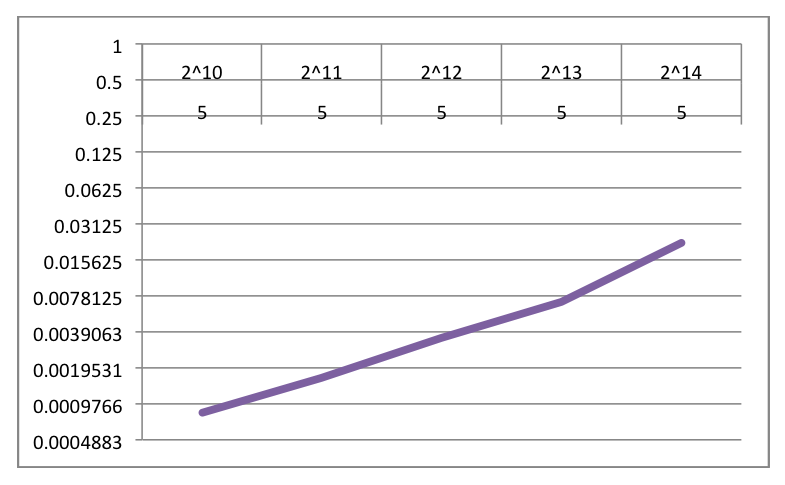
\includegraphics[scale=0.7]{BFFixedM.eps}
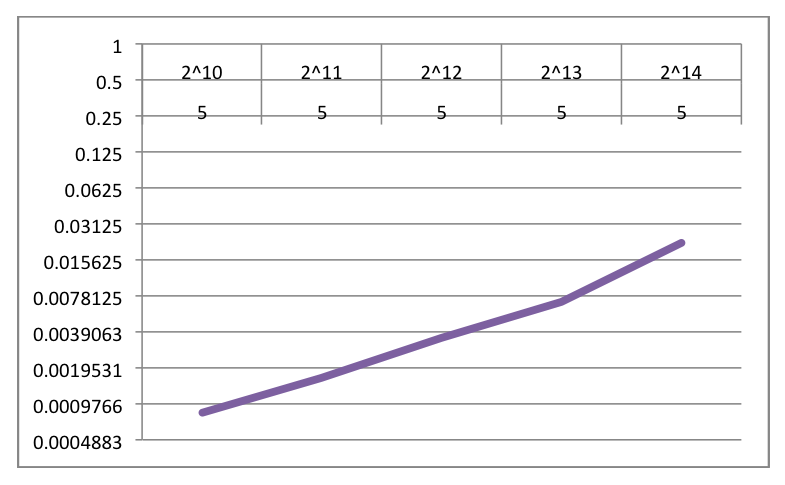
\includegraphics[scale=0.7]{BFFixedN.eps}

However, when both the pattern and text length are doubling, we see we have some order higher than $n^2$ growth of the run time, which we predicted from our complexity analysis as $n^2*m^2 > n^2$.

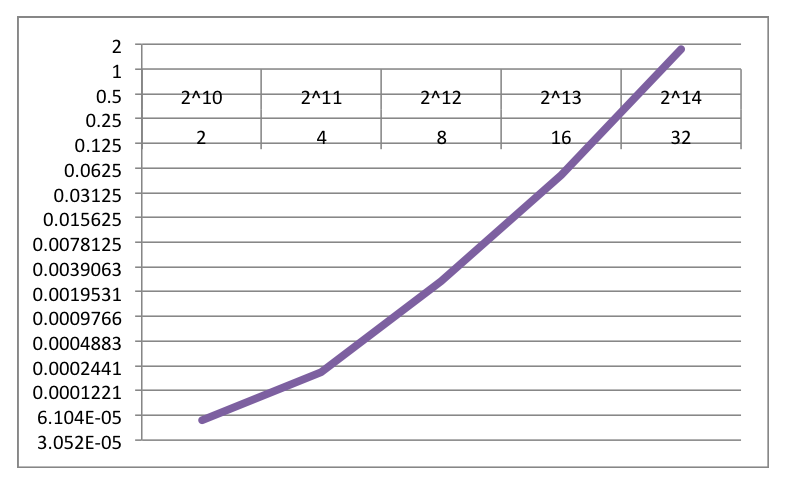
\includegraphics[scale=0.7]{BFVarM.eps}

My brute force implementation readily agrees with the literature and my earlier analysis. This is the slowest of the possible methods.

\subsubsection{ii. Knuth-Morris-Pratt}

Our first graph shows how it increases as the pattern size doubles, but the text size stays fixed. We see a very small growth, especially in comparison to the scales and slopes of the other two graphs. It's clear from this graph the match step of KMP takes the majority of the time, and it's order $O(n+m)$ is indeed equivalent to $O(n)$ as theory predicts.

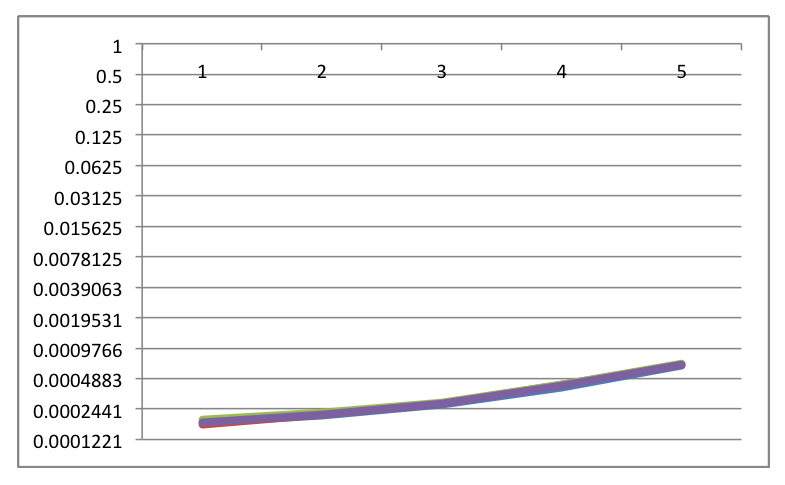
\includegraphics[scale=0.7]{KMPFixedM.eps}

The final two both double the size of text. The second one doubles the size of the pattern as well. As you can clearly see, these graphs are identical, and the preprocessing of the pattern had negligible effect on the run time.
 
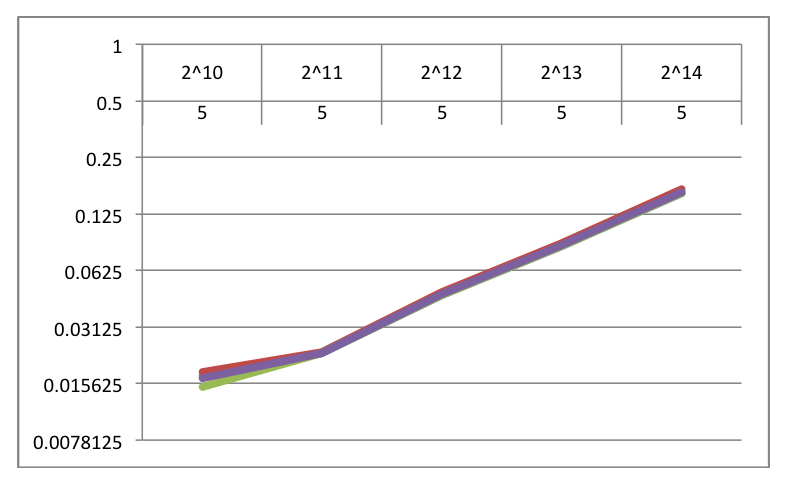
\includegraphics[scale=0.7]{KMPFixedN.eps}

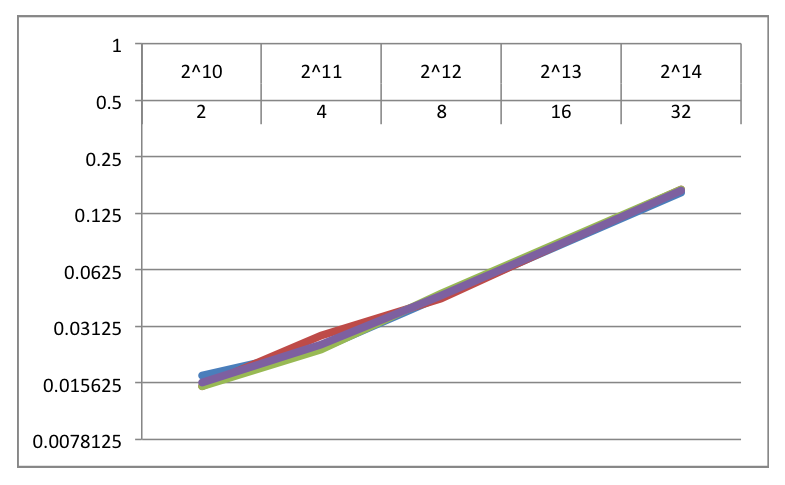
\includegraphics[scale=0.7]{KMPVar.eps}

Here I can say the performance of my implementations agrees with expected performance, and confirms my prediction of it's runtime complexity.

\subsubsection{iii. Boyer-Moore}

I was surprised by this algorithm. Our first two graphs, where we hold the text size constant and double the pattern size, and then vice versa, are virtually identical. That is, each step plays a relatively equal part in determining it's run time performance. Furthermore, my implementation on the same input performed worse on the same average input than both Brute-Force and Knuth-Morris-Pratt. 

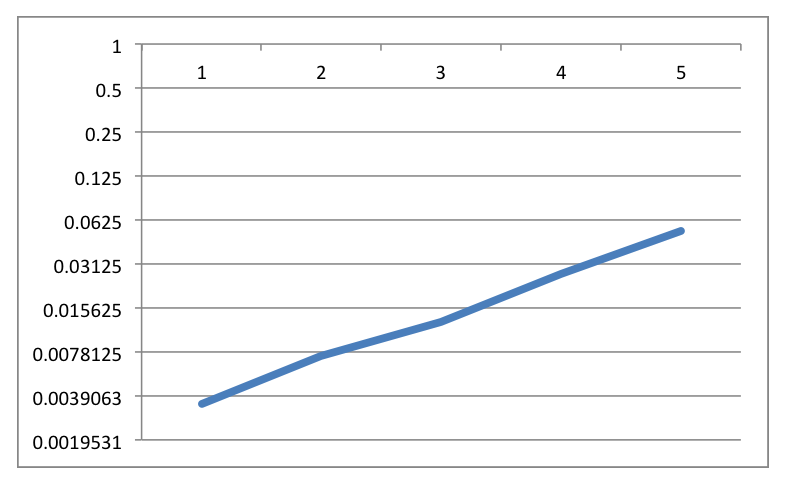
\includegraphics[scale=0.7]{BMFixedM.eps}

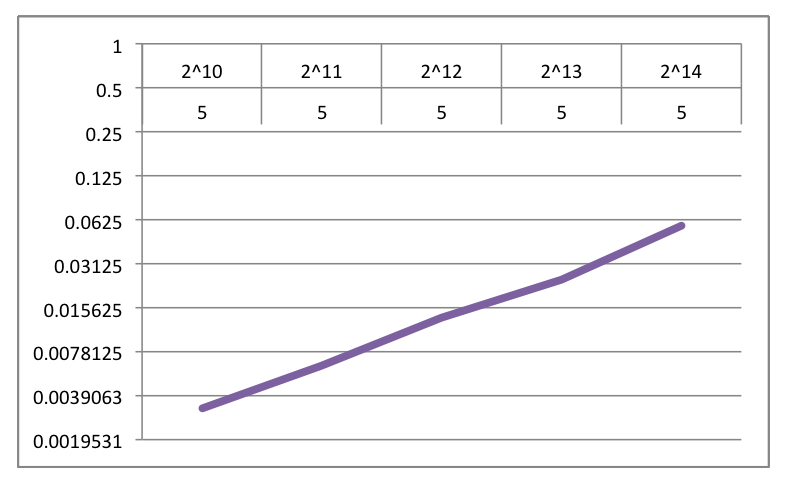
\includegraphics[scale=0.7]{BMFixedN.eps}

Here, we confirm our early observation on the graph where both inputs are doubled at each step. We see a much steeper slope than when one of the inputs was fixed. While we did beat Brute Force in this scenario at absolute performance,  complexity still seems to be in the same range, which is less than desirable.

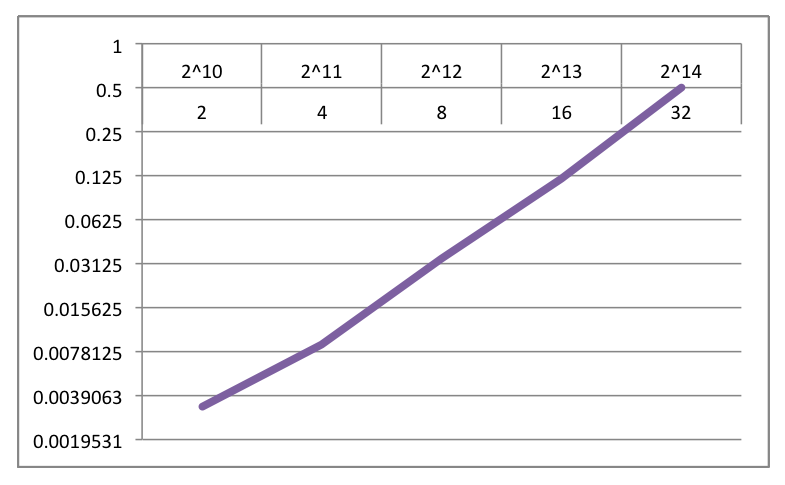
\includegraphics[scale=0.7]{BMVar.eps}

My Boyer-Moore did not agree with analysis. In fact it seemed to perform considerably worse than my analysis suggests it should. One possible explanation is my implementation of the good suffix table generation seems to make more steps than it should.

\subsubsection{iv. Rabin-Karp}

This algorithm also yielded a surprise in how slow in absolute terms it truly ran. As we see in our third graph, it took close to 10 seconds to find a pattern of length 32 in a text of length $2^14$. This is almost 5 times slower than Brute Force, and while it has nothing to say about algorithmic complexity, it's telling of how complex math is handled in a scripting language like Ruby and the real world cost to implementing this algorithm.

In our first graph, where the length of our text varies while the pattern stays constant, we see linear performance as predicted.

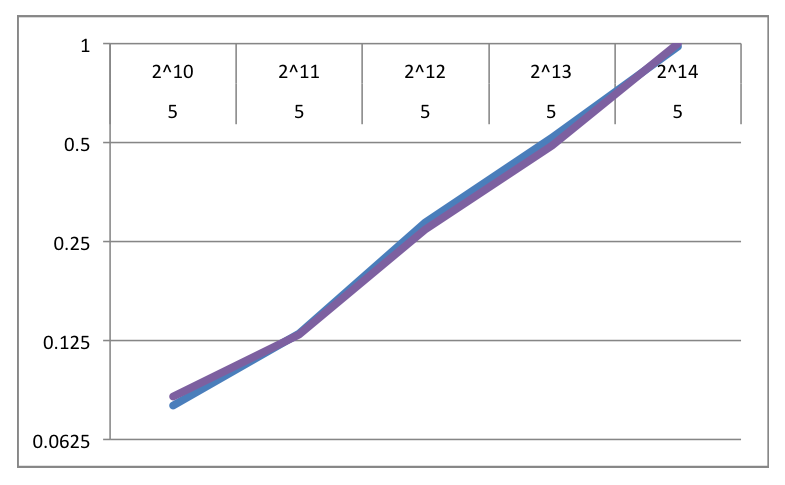
\includegraphics[scale=0.7]{RKFixedM.eps}

This second graph is our only graph not put on a $log_2$ scale, because the cost of changing the size of our pattern is actually $O(1)$. That is, the time is constant and independent of our input. This agrees with my analysis.

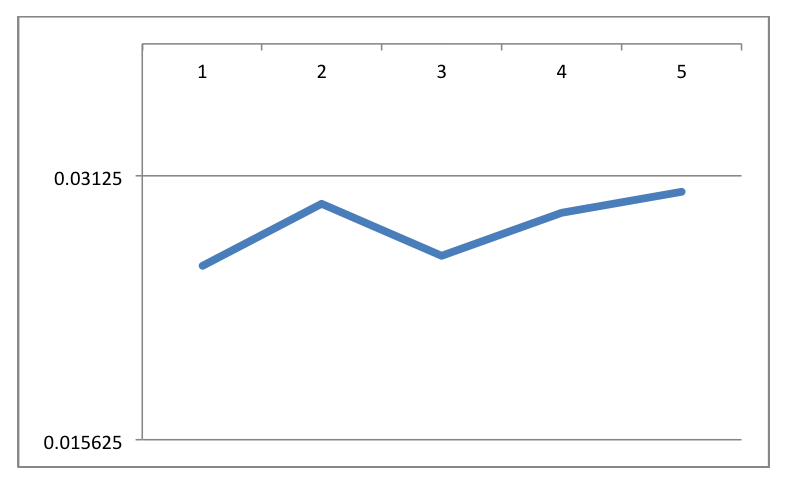
\includegraphics[scale=0.7]{RKFixedN.eps}

Finally, we see when we vary both, we got slightly higher than linear complexity. This was unpredicted and may once again come down to the difficulty in doing math on very large numbers in Ruby. 

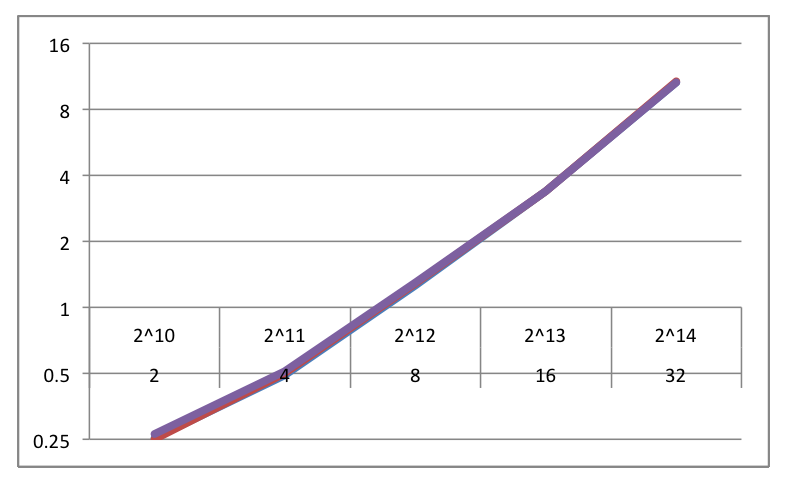
\includegraphics[scale=0.7]{RKVar.eps}

Rabin-Karp preformed worse than expected, but not drastically so when considering it's complexity. We see the hashing step is predictably constant time. The built-in string search in ruby uses this algorithm implemented in C, and performs admirably.

\subsubsection{v. Comparison}

One observation we can make is that the worse case for the brute force method also happens to be the best case for Boyer-Moore. For instance, a text that is identical for every character and a pattern that is identical to that character \emph{except} for the last character would take the maximum number of comparisons for brute force and the minimum for Boyer-Moore. We will also see best case performance in Knuth-Morris-Pratt for this case, while Rabin-Karp is simply $O(n)$. We see the results of a such a search in Table 1 with a pattern of 255 "0"'s  plus a 1 and a text of 25,600 "0"'s

\begin{table}
  \begin{center}
  \begin{tabular}{|c|c|}
  \hline
          &   \\
  {\bf Algorithm} & \parbox{1in}{\begin{center}\bf Runtime(s) \end{center}}\\
          &   \\
  \hline
          &   \\
  Brute Force  & 3.5  \\
          &   \\
  \hline
          &    \\
  Boyer-Moore & 0.13 \\
          &    \\
  \hline
          &    \\
  Knuth-Morris-Pratt & 0.03 \\
          &    \\
   \hline
          &    \\
  Rabin-Karp & 0.13 \\
          &    \\
  \hline
  \end{tabular}
  \end{center}
  \caption{Performance comparison for worst case Brute Force.}
  \label{table1}
\end{table}


\subsection{c. Space Performance}

Space performance comparison proved to be beyond my means to experimentally meaningfully measure. In Table 2, we see the approximate size in Mb that my algorithms consumed for the example input. However, the profilers output made detailed analysis too difficult to discern the difference between memory allocated to the runtime for processing and memory needed to process the strings. These figures are inexact and don't' differ in a meaningful way across inputs. For example, creation of strings often overwhelmed the memory needs of the actually algorithm and mad analysis Also, specifically the Rabin-Karp can involve large integers, and Ruby can change the size of the Integer type behind the scenes without prompting, and even switches into custom BigInteger class that spreads it across several integer types. This made understanding it's memory usage appear more as a step function than good algorithmic analysis.

\begin{table}
  \begin{center}
  \begin{tabular}{|c|c|}
  \hline
          &   \\
  {\bf Algorithm} & \parbox{1in}{\begin{center}\bf Space(Mb) \end{center}}\\
          &   \\
  \hline
          &   \\
  Brute Force  & 3.5  \\
          &   \\
  \hline
          &    \\
  Boyer-Moore & 0.13 \\
          &    \\
  \hline
          &    \\
  Knuth-Morris-Pratt & 0.03 \\
          &    \\
   \hline
          &    \\
  Rabin-Karp & 0.13 \\
          &    \\
  \hline
  \end{tabular}
  \end{center}
  \caption{Example Space comparison figures.}
  \label{table2}
\end{table}

\section{VII. Conclusion}



\newpage

\begin{thebibliography}{9}
\bibitem{lev}
Adobe Acrobat Reader 5. \\
http://www.adobe.com/products/acrobat/.

\bibitem{KMP}
Donald Knuth; James H. Morris, Jr, Vaughan Pratt (1977). \"Fast pattern matching in strings\". \\
{\em SIAM Journal on Computing} 6 (2): 323--350. 

\newpage  % to balance the columns on the last page

\bibitem{BM}
Robert S. Boyer and J. Strother Moore. (1977). A fast string searching algorithm. Commun. {\em ACM} 20, 10 (October 1977), 762--772.

\bibitem{RK}
Karp, Richard M.; Rabin, Michael O. (1987). Efficient randomized pattern-matching algorithms. {\em IBM Technical Journal} 31, (March 1987)

\end{thebibliography}
\end{document}
